\documentclass[a4paper,english]{report}

\usepackage[latin1]{inputenc}
\usepackage[T1]{fontenc}
\usepackage{fourier}
\usepackage{babel,textcomp}
\usepackage[pdftex]{graphicx}
\usepackage{subfigure}
\usepackage{listings}
\usepackage{hyperref}
\usepackage{varioref}
\usepackage{cite}
\usepackage[color]{uiosloforside}
\usepackage{tikz}
\usetikzlibrary{shapes,arrows}

\setlength\topmargin{0in}
\setlength\headheight{0in}
\setlength\headsep{0in}
\setlength\textheight{8.7in}
\setlength\textwidth{6.5in}
\setlength\oddsidemargin{0in}
\setlength\evensidemargin{0in}
\setlength\parindent{0.25in}
\setlength\parskip{0.15in}
\setlength\columnsep{0.25in}

\definecolor{dkgreen}{rgb}{0,0.6,0}
\definecolor{gray}{rgb}{0.5,0.5,0.5}
\definecolor{mauve}{rgb}{0.58,0,0.82}
\definecolor{matnat}{rgb}{0.004,0.47,0.44}

% "define" Scala
\lstdefinelanguage{scala}{
  morekeywords={abstract,case,catch,class,def,
    do,else,extends,false,final,finally,
    for,if,implicit,import,match,mixin,
    new,null,object,override,package,
    private,protected,requires,return,sealed,
    super,this,throw,trait,true,try,
    type,val,var,while,with,yield},
  otherkeywords={=>,<-,<\%,<:,>:,\#,@},
  sensitive=true,
  morecomment=[l]{//},
  morecomment=[n]{/*}{*/},
  morestring=[b]",
  morestring=[b]',
  morestring=[b]"""
}

\lstset{basicstyle=\footnotesize,
  numbers=none,
  numberstyle=\tiny\color{gray},
  keywordstyle=\color{blue},
  commentstyle=\color{dkgreen},
  stringstyle=\color{mauve},
  frame=single,
  showstringspaces=false,
  breaklines=true,
  breakatwhitespace=true,
  tabsize=3,
  language=scala
}

\hypersetup{pdfborder={0 0 0},colorlinks=true,linkcolor=blue,urlcolor=blue,citecolor=blue}

\newcommand{\matlab}{\textsc{Matlab}\textregistered}

\title{Creating high performance DSLs in Scala}
\author{Eivind Barstad Waaler (\emph{eivindwa})}

\begin{document}
\uiosloforside[kind={Master thesis},boxcolor=matnat,textcolor=white]

\chapter*{Abstract}
\addcontentsline{toc}{chapter}{Abstract}

Scala is an increasingly popular programming language running on the
JVM (Java Virtual Machine). One of its pronounced goals is to simplify
the creation of DSLs (Domain-Specific Languages) with extensible
syntax and combination of Object-Oriented and Functional
Programming. This thesis examines these possibilities with regard to
performance. It is demonstrated how you can use Scala to create
efficient DSLs on the JVM, utilizing parallel and concurrent
mechanisms found in modern computers.

\tableofcontents

\listoftables

\listoffigures

\chapter*{Preface}
\addcontentsline{toc}{chapter}{Preface}

This is a master-thesis of 60 credits\footnote{Prescribed to one year
  of full time study} in the field of Informatics. It was written for
the Object-orientation, Modelling, and Languages research
group\cite{oms} at the Department of Informatics, Faculty of
Mathematics and Natural Sciences, University of Oslo.

TODO: Thanks to supervisor++

\begin{flushright}
\textsc{Eivind Barstad Waaler}\\
Oslo, Norway\\
May 2010
\end{flushright}

\chapter{Introduction}
\label{sec:introduction}

\section{Problem Description}
\label{sec:problemdesc}

Domain Specific Languages (DSLs) are languages written to support the
implementation of problems in a specific domain or area of
interest\cite{mer05}. Scala is a relatively new programming language
being claimed to have good support for writing DSLs\cite{scala}, with
syntax that is easy to adjust and extend\cite{ode08}. Scala is also
claimed to contain powerful constructs for concurrent or parallel
programming, taking advantage of the multi-processor architectures
that are common in modern computers.

The goal of this thesis is to evaluate Scala with regards to both DSL
capabilities and parallel programming. Is it possible to combine the
scalable syntax with powerful concurrency mechanisms to create ``High
Performance DSLs in Scala''?

\section{Method}
\label{sec:method}

This section describes the research methods applied in this
thesis. In\cite{dyb08} the concept ``Evidence-Based Software
Engineering'' (EBSE) is introduced. Although this article is mainly
targeted towards practicioners looking to support decision-making I
feel that it gives a good foundation for evaluating research methods
related to Software Engineering. The main steps of EBSE are as
follows:

\begin{enumerate}
\item Convert a relevant problem or need for information into an
  answerable question.
\item Search the literature for the best available evidence to answer
  the question.
\item Critically appraise the evidence for its validity, impact, and
  applicability.
\item Integrate the appraised evidence with practical experience and
  the client's values and circumstances to make decisions about
  practice.
\item Evaluate performance in comparison with previous performance and
  seek ways to improve it.
\end{enumerate}

With this list as basis I ended up with the following steps for this
thesis:

\begin{enumerate}
\item Create answerable questions -- Make sure the questions to
  research are sound and possible to answer.
\item Search existing literature -- Find literature to provide direct
  answers to the questions, or to support assumptions needed to
  sustain experiments.
\item Critically appraise the literature evidence -- Make sure the
  chosen literature actually provide valid evidence for its claims.
\item Conduct experiments -- The major part of the thesis work is of
  course related to the experiments conducted. The first three steps
  are important to make sure the experiments are based on sound
  evidence and former knowledge.
\item Critical evaluation -- The experiments and results found must be
  carefully evaluated. By being critical to my own results I hope to
  improve the overall quality of the thesis deliverance.
\end{enumerate}

\chapter{Domain Specific Languages}
\label{sec:dsls}

\textit{``Domain-specific languages (DSLs) are languages tailored to a
  specific application domain. They offer substantial gains in
  expressiveness and ease of use compared with general-purpose
  programming languages.''}\cite{mer05}

We have two main types of DSLs; internal and external DSLs. Internal
DSLs uses the host language so that it gets the feel of a particular
language. They are compiled and run together with the host
language. Internal DSLs are also referred to as embedded DSLs or
Fluent Interfaces. Internal DSLs have custom syntax and typically
requires you to write a full parser to process them.

Scala has features to support development of both internal and
external DSLs. They will be described in the following sections.

\chapter{Scala}
\label{sec:scala}

\textit{``Scala is a general purpose programming language designed to
  express common programming patterns in a concise, elegant, and
  type-safe way. It smoothly integrates features of object-oriented
  and functional languages, enabling Java and other programmers to be
  more productive. Code sizes are typically reduced by a factor of two
  to three when compared to an equivalent Java
  application''.}\cite{scala}

Scala is a relatively new language (first version released
2003\cite{scala}) providing exciting programming capabilities on the
Java Virtual Machine (JVM). The main reason for chosing Scala in this
thesis is the combination of powerful programming structures (both
object-oriented and functional) with the cross-platform and wide
adoption of the JVM. Code written in Scala can be run on any JVM
version 1.5 or newer, and can utilize any library written in Java. It
can thus be seen as a <<best of both worlds>> language.

The following sections describe properties of Scala that might make it
suited for building <<high performance DLSs>> on the JVM. For more
detailed information about Scala please refer
to\cite{ode08},\cite{scala} or\cite{scalatour}.

\section{Scala and Java}
\label{sec:scalajava}

Scala code (.scala files) compiles to Java bytecode (.class files)
through a special compiler (\texttt{scalac}). The bytecode can then be
run on the JVM as if it was created from Java source (.java files). In
adition Scala provides a number of library classes that need to be
included as a jar file. This relationship between Scala and Java is
illustrated in figure \vref{fig:scalajava}.

\begin{figure}
  \begin{center}
  \tikzstyle{block} = [rectangle, draw, fill=blue!20, text width=5em, text centered, rounded corners, minimum height=4em]
  \tikzstyle{line} = [draw, -latex']
  \tikzstyle{cloud} = [draw, ellipse,fill=red!20, text width=5em, text centered, node distance=2.5cm, minimum height=2em]
  \begin{tikzpicture}[node distance = 2cm, auto]
    % Place nodes
    \node [cloud] (class) {Java Bytecode (.class)};
    \node [block, left of=class, above of=class] (scalacompile) {Scala Compile (scalac)};
    \node [cloud, left of=scalacompile] (scala) {Scala Source (.scala)};
    \node [block, right of=class, above of=class] (javacompile) {Java Compile (javac)};
    \node [cloud, right of=javacompile] (java) {Java Source (.java)};
    \node [block, below of=class] (jvm) {Java Virtual Machine};
    \node [block, below of=scala] (scalalib) {Scala API (.jar)};
    % Draw edges
    \path [line] (scalacompile) -- (class);
    \path [line] (javacompile) -- (class);
    \path [line] (class) -- (jvm);
    \path [line] (scala) -- (scalacompile);
    \path [line] (java) -- (javacompile);
    \path [dotted, line] (scalalib) -- (jvm);
  \end{tikzpicture}
  \end{center}
  \caption{Visual representation of the relationship between Scala and
    Java.\label{fig:scalajava}}
\end{figure}

The tight relationship with Java has a number of advantages when using
Scala:

\begin{itemize}
\item Cross-platform distribution -- Code written in Scala can be run
  on any platform supporting JVM 1.5 or newer.
\item Stability and standards -- The JVM is a stable platform with
  good support for internationalization (Unicode support ++) and
  localization (supports local languages and standards).
\item Access to libraries -- The JVM has a wide range of libraries
  available, many being Open Source.
\item High performance -- The JVM has been proven to be a high
  performant Virtual Machine, with a large number of tuning
  possibilities.
\end{itemize}

There are also disadvantages with such a tight coupling to the JVM:

\begin{itemize}
\item Limitations in bytecode -- Scala, being a functional language,
  would benefit from features not present in the current version of
  the JVM. Most notably is the (lack of) support for full tail call
  optimization, which would improve performance of recursive
  functions.
\item Generics implemented with erasure -- Scala uses an erasure
  scheme to implement generics, to be 100\% compatible with
  Java. However, the implementation of the Scala compiler
  (\texttt{scalac}) has some advanced solution to many of the problems
  Java has regarding erasure\cite{emi06}.
\end{itemize}

\section{DSL capabilities in Scala}
\label{scaladsl}

This section describes some features and properties of Scala with
regard to DSL creation. The first sub sections describe properties
related to internal DSL building, while section \vref{sec:combparse}
describes <<Combinator Parsers>> which is a feature used to create
external DSLs.

\subsection{Type Inference and Implicits}

The Scala compiler will try to infer the types used. So if the type is
obvious there is no need to specify it:

\begin{lstlisting}
val i = 42 // Type Int is infered
val d = i + 2.1 // Type Double is infered
\end{lstlisting}

The language also supports implicit type conversions. So if an object
does not have the method being called on it, the compiler will try to
convert it to a type that contains the method:

\begin{lstlisting}
// Wrapper class for int
class MyInt(val i: Int) {
  def doubleIt = i * 2 // Method
}
// Implicit conversion
implicit def fromInt(i: Int) = new MyInt(i)
// Convert Int to MyInt and call method
4.doubleIt
\end{lstlisting}

\subsection{Method Names and Operator Notation}

Scala has two features regarding method names and syntax that are
interesting with regards to DSL development:

\begin{itemize}
\item Arbitrary method names - Scala methods can have special
  characters as names. As such Scala has full support for operator
  overloading, as operators are just regular methods with special
  names. For example \texttt{+}, \texttt{!=} and \texttt{<=}.
\item Operator notation - Methods in Scala can be called without the
  dot and parentheses, as shown in the examples below.
\end{itemize}

\begin{lstlisting}
abstract class Matrix {
  // Method names can be operators
  def +(other: Matrix) = add(other)
  // Regular method name
  def add(other: Matrix): Matrix
}
// Regular notation
val m3 = m1.+(m2)
val m3 = m1.add(m2)
// Operator notation
val m3 = m1 + m2
val m3 = m1 add m2
\end{lstlisting}

\subsection{The ``magic'' \texttt{apply} Method}

Scala uses the \texttt{apply} method to let classes and object define
functionality that appears to be native in the language. In the
following example the \texttt{apply} method is used to index the
\texttt{Matrix} class as if it was a native feature:

\begin{lstlisting}
class Matrix[T] {
  def apply(row: Int, col: Int): T = ...
}
val intMatrix = ... // Matrix[Int]
// Get Int at position 2, 4
val intVal = intMatrix(2, 4)
\end{lstlisting}

\subsection{Traits - Polymorphic Abilities}

Scala has support for virtual types (abstract type members) and
familiy polymorphism\cite{ode03}, mixin composition\cite{ode05} and
higher-order genericity\cite{moo08}. These are all powerful features
that support polymorphic embedding of DSLs\cite{hof08}.

This allows building DSLs that can have several different
interpretations as reusable components. It can also be used to
effectively combine different DSLs into new ones. The paper
``Polymorphic Embedding of DSLs''\cite{hof08} describes this in detail
with examples.

A use of traits can be to split functionality in several traits and
create classes/objects with only the methods that we need. In the
following example the \texttt{Matrix} class does not have any methods,
but instances of the class can be mixed in with traits containing
various methods:

\begin{lstlisting}
class Matrix {} // No methods

trait AvgMtx { this: Matrix =>
  def avg(): Matrix = { ... }
}

trait MorphMtx { this: Matrix =>
  def erode(): Matrix = { ... }
  def dilate(): Matrix = { ... }
}

// Matrix with only avg() method
val m1 = new Matrix with AvgMtx
// Matrix with erode() and dilate() methods
val m2 = new Matrix with MorphMtx
// Matrix with "all" methods
val m3 = new Matrix with AvgMtx with MorphMtx
\end{lstlisting}

\subsection{Combinator Parsing}
\label{sec:combparse}

Scala includes a library for building parser combinators - functions
and operators defined in Scala that will serve as building blocks for
parsers. The mechanism is described in detail in chapter 31 in the
``Programming in Scala'' book\cite{ode08}.

Simply explained this allows a developer to specify a grammar with
actions directly in Scala, thus building support for an internal
DSL. The example below show a simple grammar for arithmetic
expressions:

\begin{lstlisting}
import scala.util.parsing.combinator._ 

// Simple arithmetic parser
class Arith extends JavaTokenParsers { 
  def expr: Parser[Any] =
    term~rep("+"~term | "-"~term) 
  def term: Parser[Any] =
    factor~rep("*"~factor | "/"~factor) 
  def factor: Parser[Any] =
    floatingPointNumber | "("~expr~")" 
}

// Testing the parser
val parser = new Arith
val input = "2 * (4 + 5)" // OK input
println(parser.parseAll(parser.expr, input))
val bad = "2 * ((4 + 5)" // Bad parenthesis
println(parser.parseAll(parser.expr, bad))
\end{lstlisting}

The example does not perform any actions, but still shows how the
mechanism works. The first example passes ok and the second one yields
an error as it is missing a parenthesis:

\begin{lstlisting}[language=tex]
parser.parseAll(parser.expr, bad)

[1.13] failure: `)' expected but `' found

2 * ((4 + 5)
            ^
\end{lstlisting}

A simplified version of the above example implemented with actions
could look as follows:

\begin{lstlisting}
import scala.util.parsing.combinator._

class Arith extends JavaTokenParsers {
  def expr: Parser[Double] =
    factor~"+"~factor ^^ 
      { case f1~"+"~f2 => f1 + f2 }
  def factor: Parser[Double] =
    floatingPointNumber ^^ (_.toDouble)
}

// Testing
val p = new Arith
val parse = p.parseAll(p.expr, _: String).get
println(parse("2 + 3")) // Output: 5.0
println(parse("2.5 + 3.1")) // Output: 5.6
\end{lstlisting}

In this example the grammar is simple enough to evaluate directly in
the actions. It would be easy to create a separate evaluation system
instead. However it is implemented this allows for using the
combinator parsing framework to embed an external DSL directly in the
language.

\chapter{Results}

\section{DSL for Image Processing}

\subsection{Description}

Image Processing is an area involving series of computationally heavy
operations performed on images. Many practicioners in the area have
more mathematical than computer science oriented background. This
leads to the need for DSLs where complicated and computationally heavy
operations can be performed with a simple and straightforward syntax.

A major actor in the art of Image Processing is the product \matlab
from the company MathWorks\texttrademark. They provide the user with a
DSL for doing advanced Image Processing operations. I have tried to
create a similar DSL (with limited functionality) in Scala.

As an example consider the operation of blurring an image using an
average filter mask show in figures \vref{fig:eximg} and
\vref{fig:exavg}. This is a basic operation, but serves good as an
example of using the DSLs.

The \matlab{} code to perform the operation could
typically look like this:
\begin{lstlisting}[language=matlab]
img = imread('cell.jpg');
% 3x3 neighborhood default
imgAvg = medfilt2(img);
imwrite(imgAvg, 'cell_avg.jpg');
\end{lstlisting}

My goal is to create a Scala DSL to achieve the same result. A
suggested Scala-solution to the problem will look something like this:

\begin{lstlisting}
// Imports...
val img = loadImageCP("/cell.jpg")
val se = StrEl(Square, 3)
val imgAvg = img.avg(se)
saveImage(imgAvg, "/cell_avg.jpg")
\end{lstlisting}

\begin{figure}
  \subfigure[Original]{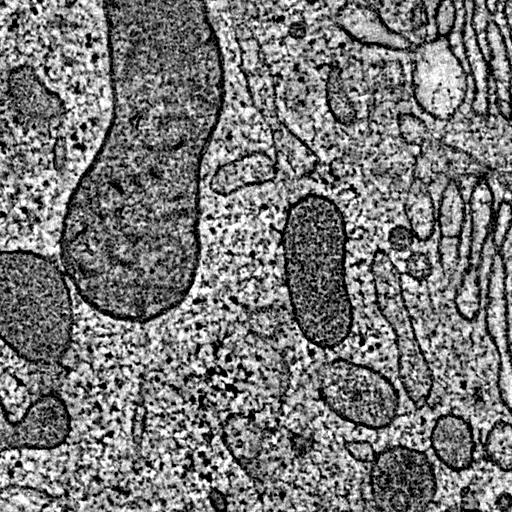
\includegraphics[width=0.49\textwidth]{images/cell}}
  \hfill
  \subfigure[Blurred]{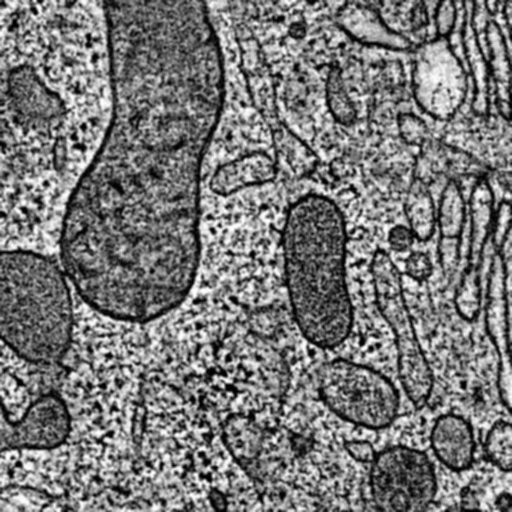
\includegraphics[width=0.49\textwidth]{images/cell_avg}}
  \caption{Example image before and after blurring with average
    filter.\label{fig:eximg}}
\end{figure}

\begin{figure}
  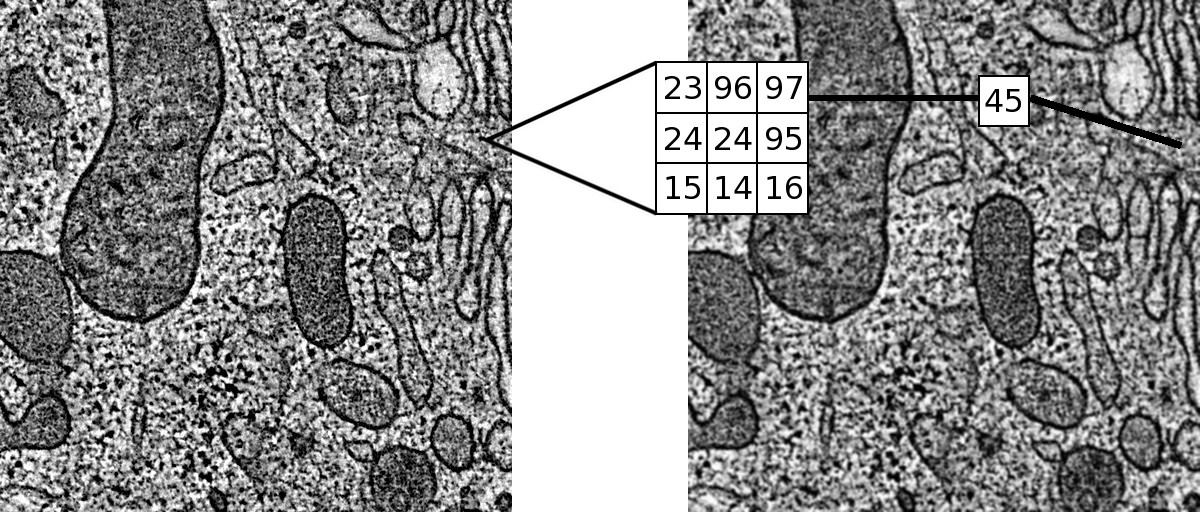
\includegraphics[width=1.0\textwidth]{images/avg_process}
  \caption{Visualising the process of blurring an image using average
    filtering with a 3x3 neighbourhood.\label{fig:exavg}}
\end{figure}

The rest of this section describes how I implemented this, and what
the results where with regards to the performance (how efficient the
implementation is).

\subsection{Syntax}

Importing members for easy access:

\begin{lstlisting}
import io.SImageIO._
import structs.StrElType._

// SImageIO.loadImageCP("/cell.jpg")
val img = loadImageCP("/cell.jpg")
...
saveImage(imgAvg, "/cell_avg.jpg")

// StrElType.Square
val se = StrEl(Square, 3)
\end{lstlisting}

Using singleton objects as factories:

\begin{lstlisting}
object StrEl {
  import StrElType._
  def apply(t: StrElType, num: Int) = Array2DStrEl(t, num)
}

val se = StrEl(Square, 3)
\end{lstlisting}

Using Traits to add operations. Optionally using operator notation:

\begin{lstlisting}
trait Standard { this: GrayScaleImage =>
  def avg(se: StrEl[Int]) = { ... }
}

object Image {
  import operations.{Morphology, Standard}

  def apply(d: Matrix[Int]) = {
    new GrayScaleImage(d) with Standard with Morphology
  }
}

val imgAvg = img.avg(se)

// Equivalent - operator notation
val imgAvg = img avg se
\end{lstlisting}

\subsection{Parallel Processing}

With images larger than a certain size, the operations performed in
the image analysis are bound to be heavy in terms of the number of
computations that need to be executed. This opens up a demand for
exploiting the capabilities found in modern computers with regard to
parallelization and concurrency. In the following sections we look at
different mechanisms available from the Scala language to achieve
better performance through utilization of the hardware resources
available in the computer. The first two sections discuss mechanisms
for concurrent programming on a multi-core/-processor environment,
while the third section discuss a mechanism for parallelization using
the GPU (Graphics Processing Unit).

\subsubsection{Actors API}
\label{sec:actors}

Describe Actors API with example from DSL.

\subsubsection{Futures API}
\label{sec:futures}

Describe Futures API with example from DSL.

\subsubsection{OpenCL with ScalaCL}
\label{sec:opencl}

Brief description of OpenCL\cite{opencl} and ScalaCL\cite{scalacl}.

Description of DSL example using ScalaCL.

\subsection{Efficient Implementation Tips}
\label{sec:effimpl}

When performing the same operation a large number of times, as is the
case with many algorithms for Image Processing, there are various
implementation related things that need to be considered. In this
section I summarize the lessons learned with regards to tuning the
code for maximum performance.

\subsubsection{Choice of data structures}
\label{sec:datastructures}

The underlying data structure for images and Image Processing is the
matrix. Since Scala does not include an efficient implementation of
matrix I ended up testing a few different variants:

\begin{itemize}
\item \textbf{List of Lists} -- A very logical implementation of
  matrix is by using Scala \texttt{Lists}. The idea for this
  implementation was inspired by a blog post by Jonathan
  Merritt\cite{mer08}. A simple example of using a list of lists is
  shown in figure \vref{fig:listoflist}. However, this implementation
  proves to be very slow in specific element access and iteration.
\item \textbf{2D Array} -- In Scala an \texttt{Array} will usually be
  faster than \texttt{List} because it is compiled to a native array
  in bytecode. It is also faster to implement as one flat array,
  rather than an array of arrays. This gives a much more efficient
  implementation with regards to element access and iteration. The
  implementation becomes slightly less straight-forward as we need to
  calculate the element positions in the array, as shown in figure
  \vref{fig:2darray}.
\end{itemize}

\begin{figure}
  \begin{lstlisting}
class Matrix[T](val elements: List[List[T]]) {
  val nRows = elements.size
  val nCols = if(elements.isEmpty) 0
              else elements.head.size

  require(elements.forall(_.length == nCols))

  def apply(row: Int, col: Int): T = elements(row)(col)
}

val m = new Matrix(List(List(1, 2), List(3, 4)))
  \end{lstlisting}
  \caption{Matrix implementation based on List of
    Lists.\label{fig:listoflist}}
\end{figure}

\begin{figure}
  \begin{lstlisting}
class Matrix[T](cols: Int, val elements: Array[T]) {
  require(elements.size % cols == 0)

  val nRows = elements.size / cols
  val nCols = cols

  def apply(row: Int, col: Int): T = elements(col + row * nCols)
}

val m = new Matrix(2, Array(1, 2, 3, 4))
  \end{lstlisting}
  \caption{Matrix implementation based on 2D
    Array.\label{fig:2darray}}
\end{figure}

\subsubsection{Iterations -- \texttt{for} comprehensions vs \texttt{while} loops}

Many Image Processing operations require some kind of calculation
performed for every element in the underlying matrix. As an example,
consider the neighbour average operation implemented using a general
structuring-element operation show in figure
\vref{fig:strelavg}. Having as efficient implementation of the
\texttt{seOp} method as possible is critical for large matrices. So
having some way of efficiently iterating over all elements of the
matrix is essential. Scala provides two basic forms of iterating;
\texttt{for comprehensions} and \texttt{while loops}:

\begin{itemize}
\item \textbf{for comprehensions} -- In Scala, for comprehensions are
  implemented as a monadic combination of the methods \texttt{filter},
  \texttt{map} and \texttt{flatMap}. This is a very powerful structure
  allowing compact and readable code. An example of implementing a
  general structuring-element operation based on for comprehensions is
  show in figure \vref{fig:forcomp}.
\item \textbf{while loops} -- For regular loops Scala provides the
  \texttt{while} keyword. Using this instead of the for comprehensions
  gives a much more iterative implementation, as shown in figure
  \vref{fig:whileloop}.
\end{itemize}

\begin{figure}
  \begin{lstlisting}
class Matrix ... {
  def seOp(se: Matrix, op: (Seq[Int]) => Int) = { ... }
}

val matrix = ... // Create matrix - load image or similar
val se = new Matrix(3, Array.make(9, 1))
val avgMatrix = matrix.seOp(se, (seq) => seq.reduceLeft(_ + _) / seq.size)
  \end{lstlisting}
  \caption{Implementing matrix neighbour average using a general
    structuring-element operation.\label{fig:strelavg}}
\end{figure}

\begin{figure}
  \begin{lstlisting}
def seOp(se: Matrix, op: (Seq[Int]) => Int) = {
  val w = se.nCols / 2
  val h = se.nRows / 2

  def seValues(row: Int, col: Int) = {
    for {
      x <- -w to w
      cx = col + x
      y <- -h to h
      ry = row + y
      if(cx >= 0 && cx < nCols && ry >= 0 && ry < nRows)
    } yield {
      elements(cx + ry * nCols)
    }
  }
  val range = for(i <- 0 until nRows; j <- 0 until nCols) yield {
    op(seValues(i, j))
  }
  new Matrix(nCols, range.toArray)
}
  \end{lstlisting}
  \caption{Implementation of a structuring element operation on a
    matrix using \texttt{for comprehensions}.\label{fig:forcomp}}
\end{figure}

\begin{figure}
  \begin{lstlisting}
def seOp(se: Matrix, op: (Seq[Int]) => Int) = {
  val w = se.nCols / 2
  val h = se.nRows / 2

  val newArr = Array.make(arr.size, 0)
  var points: List[Int] = Nil
  var j, i, x, y, cx, ry = 0
  while(j < nCols) {
    i = 0
    while(i < nRows) {
      points = Nil
      x = -w
      while(x <= w) {
        cx = i + x
        y = -h
        while(y <= h) {
          ry = j + y
          if(cx >= 0 && cx < nCols && ry >= 0 && ry < nRows) {
            points = elements(cx + ry * nCols) :: points
          }
          y = y + 1
        }
        x = x + 1
      }
      newArr(i + j * nCols) = op(points)
      i = i + 1
    }
    j = j + 1
  }
  new Matrix(nCols, newArr)
}
  \end{lstlisting}
  \caption{Implementation of a structuring element operation on a
    matrix using \texttt{while loops}.\label{fig:whileloop}}
\end{figure}

\begin{itemize}
  \item Scala and primitives
  \item JVM tuning
\end{itemize}

\begin{table}[ht]
  \centering
  \begin{tabular}{c c c c}
    \hline\hline
    & find & addlast & delfirst \\ [0.5ex]
    \hline\hline
    find & OK & I & I \\
    addlast & - & I & I \\
    delfirst & - & - & I \\
    \hline\hline
  \end{tabular}
  \caption{A pure example table.\label{tab:ex1}}
\end{table}

\chapter{Summary}

Summary.. $\ddot\smile$

\addcontentsline{toc}{chapter}{Bibliography}
\bibliography{master}
\bibliographystyle{plain}

\end{document}
